\documentclass[../../main.tex]{subfiles}

\graphicspath{{images/Maschinentechnik/}{../../images/Maschinentechnik/}}

\lstset{basicstyle=\small,
      showstringspaces=false,
      commentstyle=\color{black},
      keywordstyle=\color{blue}
    }

\begin{document}

\subsection{Inbetriebnahme Mechanik}

Die Bedienung der Lokomotive ''Soultrain'' kann in vier einfachen Teilschritten vorgenommen werden:\\

\textbf{1. Lokomotive auf die Gleise stellen}\\
Die Lokomotive soll innerhalb des Startbereichs auf die Gleise gestellt werden und korrekt auf allen Rädern aufliegen.
Es ist darauf zu achten, dass die Schleifkontakte die Gleise richtig berühren und die nötige Vorstannung aufweisen.

\begin{figure}[H]
  \centering
  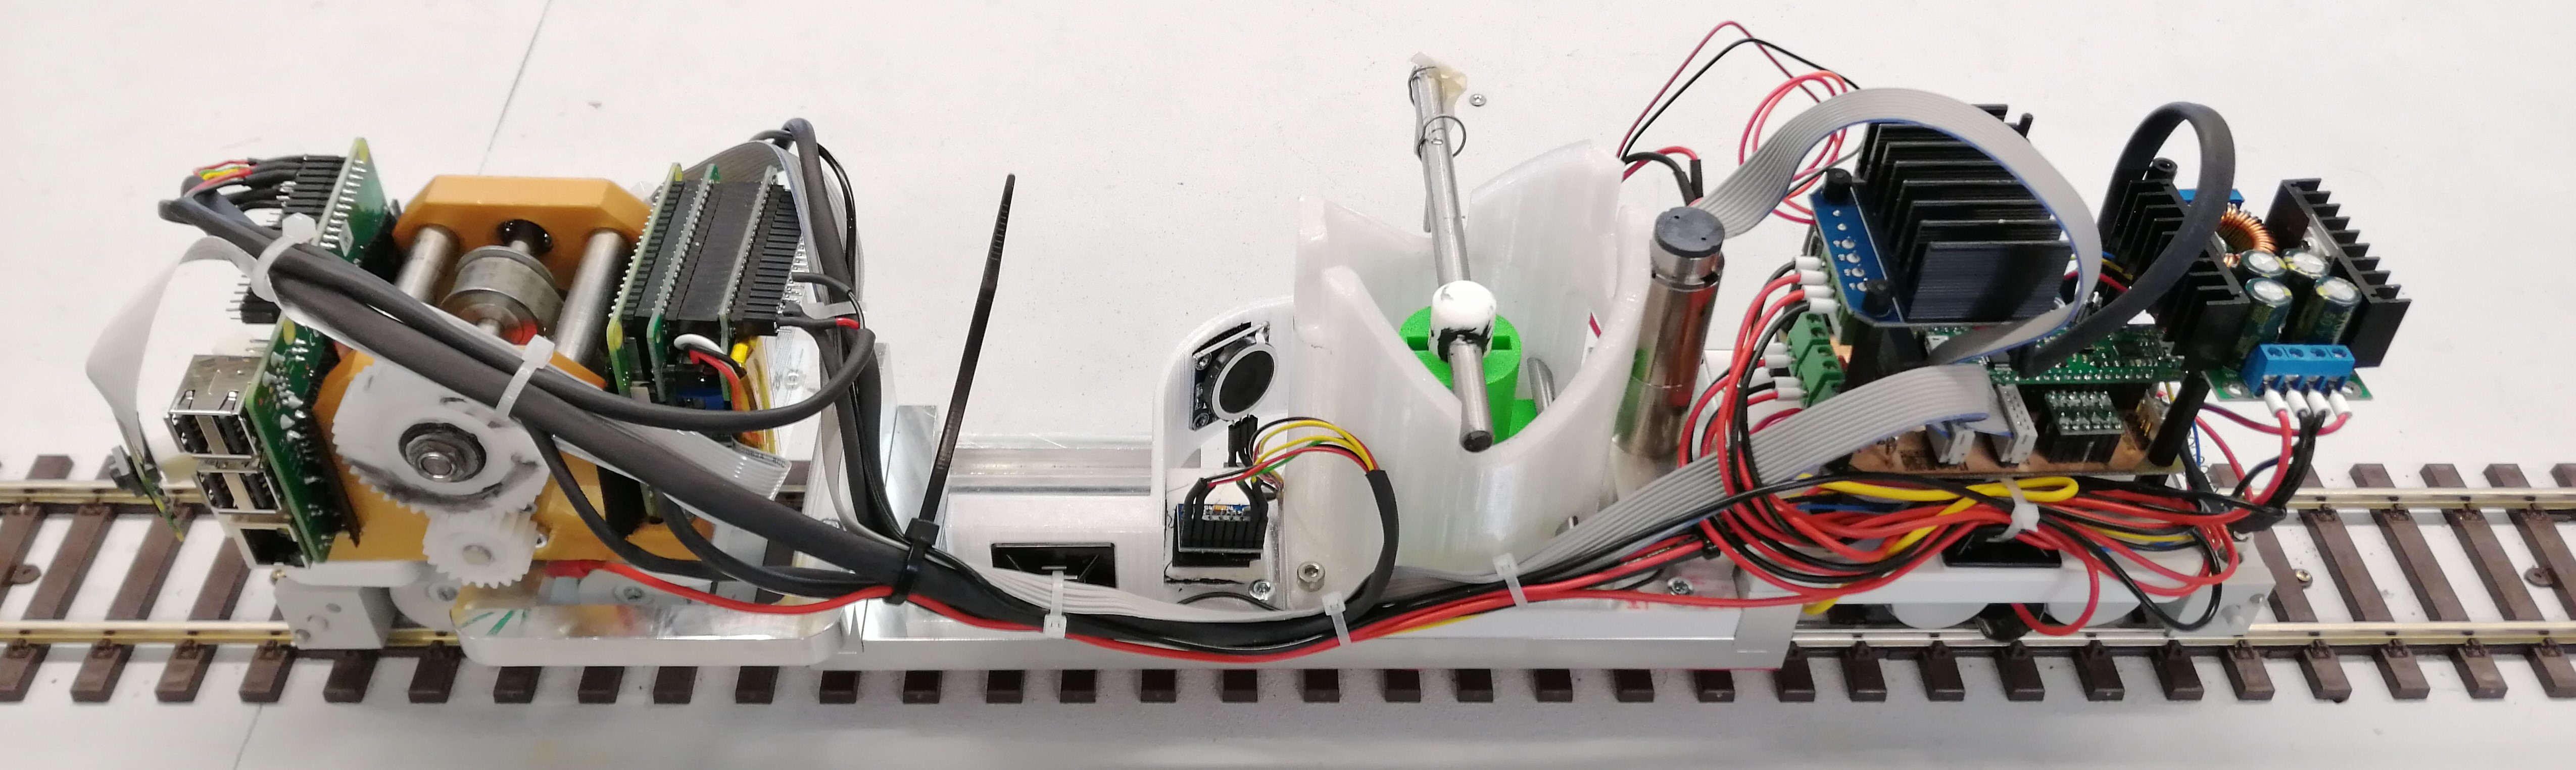
\includegraphics[width=1\textwidth]{montagezug.PNG}
  \caption {Lokomotive auf die Gleise stellen}
  \label{fig:montagezug}
\end{figure}

\textbf{2. Kurvenvorrichtung hinten und vorne von der Lokomotive einhacken}\\
Die Zapfen an beiden Enden müssen hineingedrückt werden, um die Vorrichtung korrekt in die Gleise einzuhacken. Es ist darauf zu achten, dass die Kontur der Stahlstifte korrekt an derer der Gleise ausgerichtet ist.\\
Dieser Arbeitsschritt muss vorne wie auch hinten an der Lokomotive ausgeführt werden.

\begin{figure}[H]
  \centering
  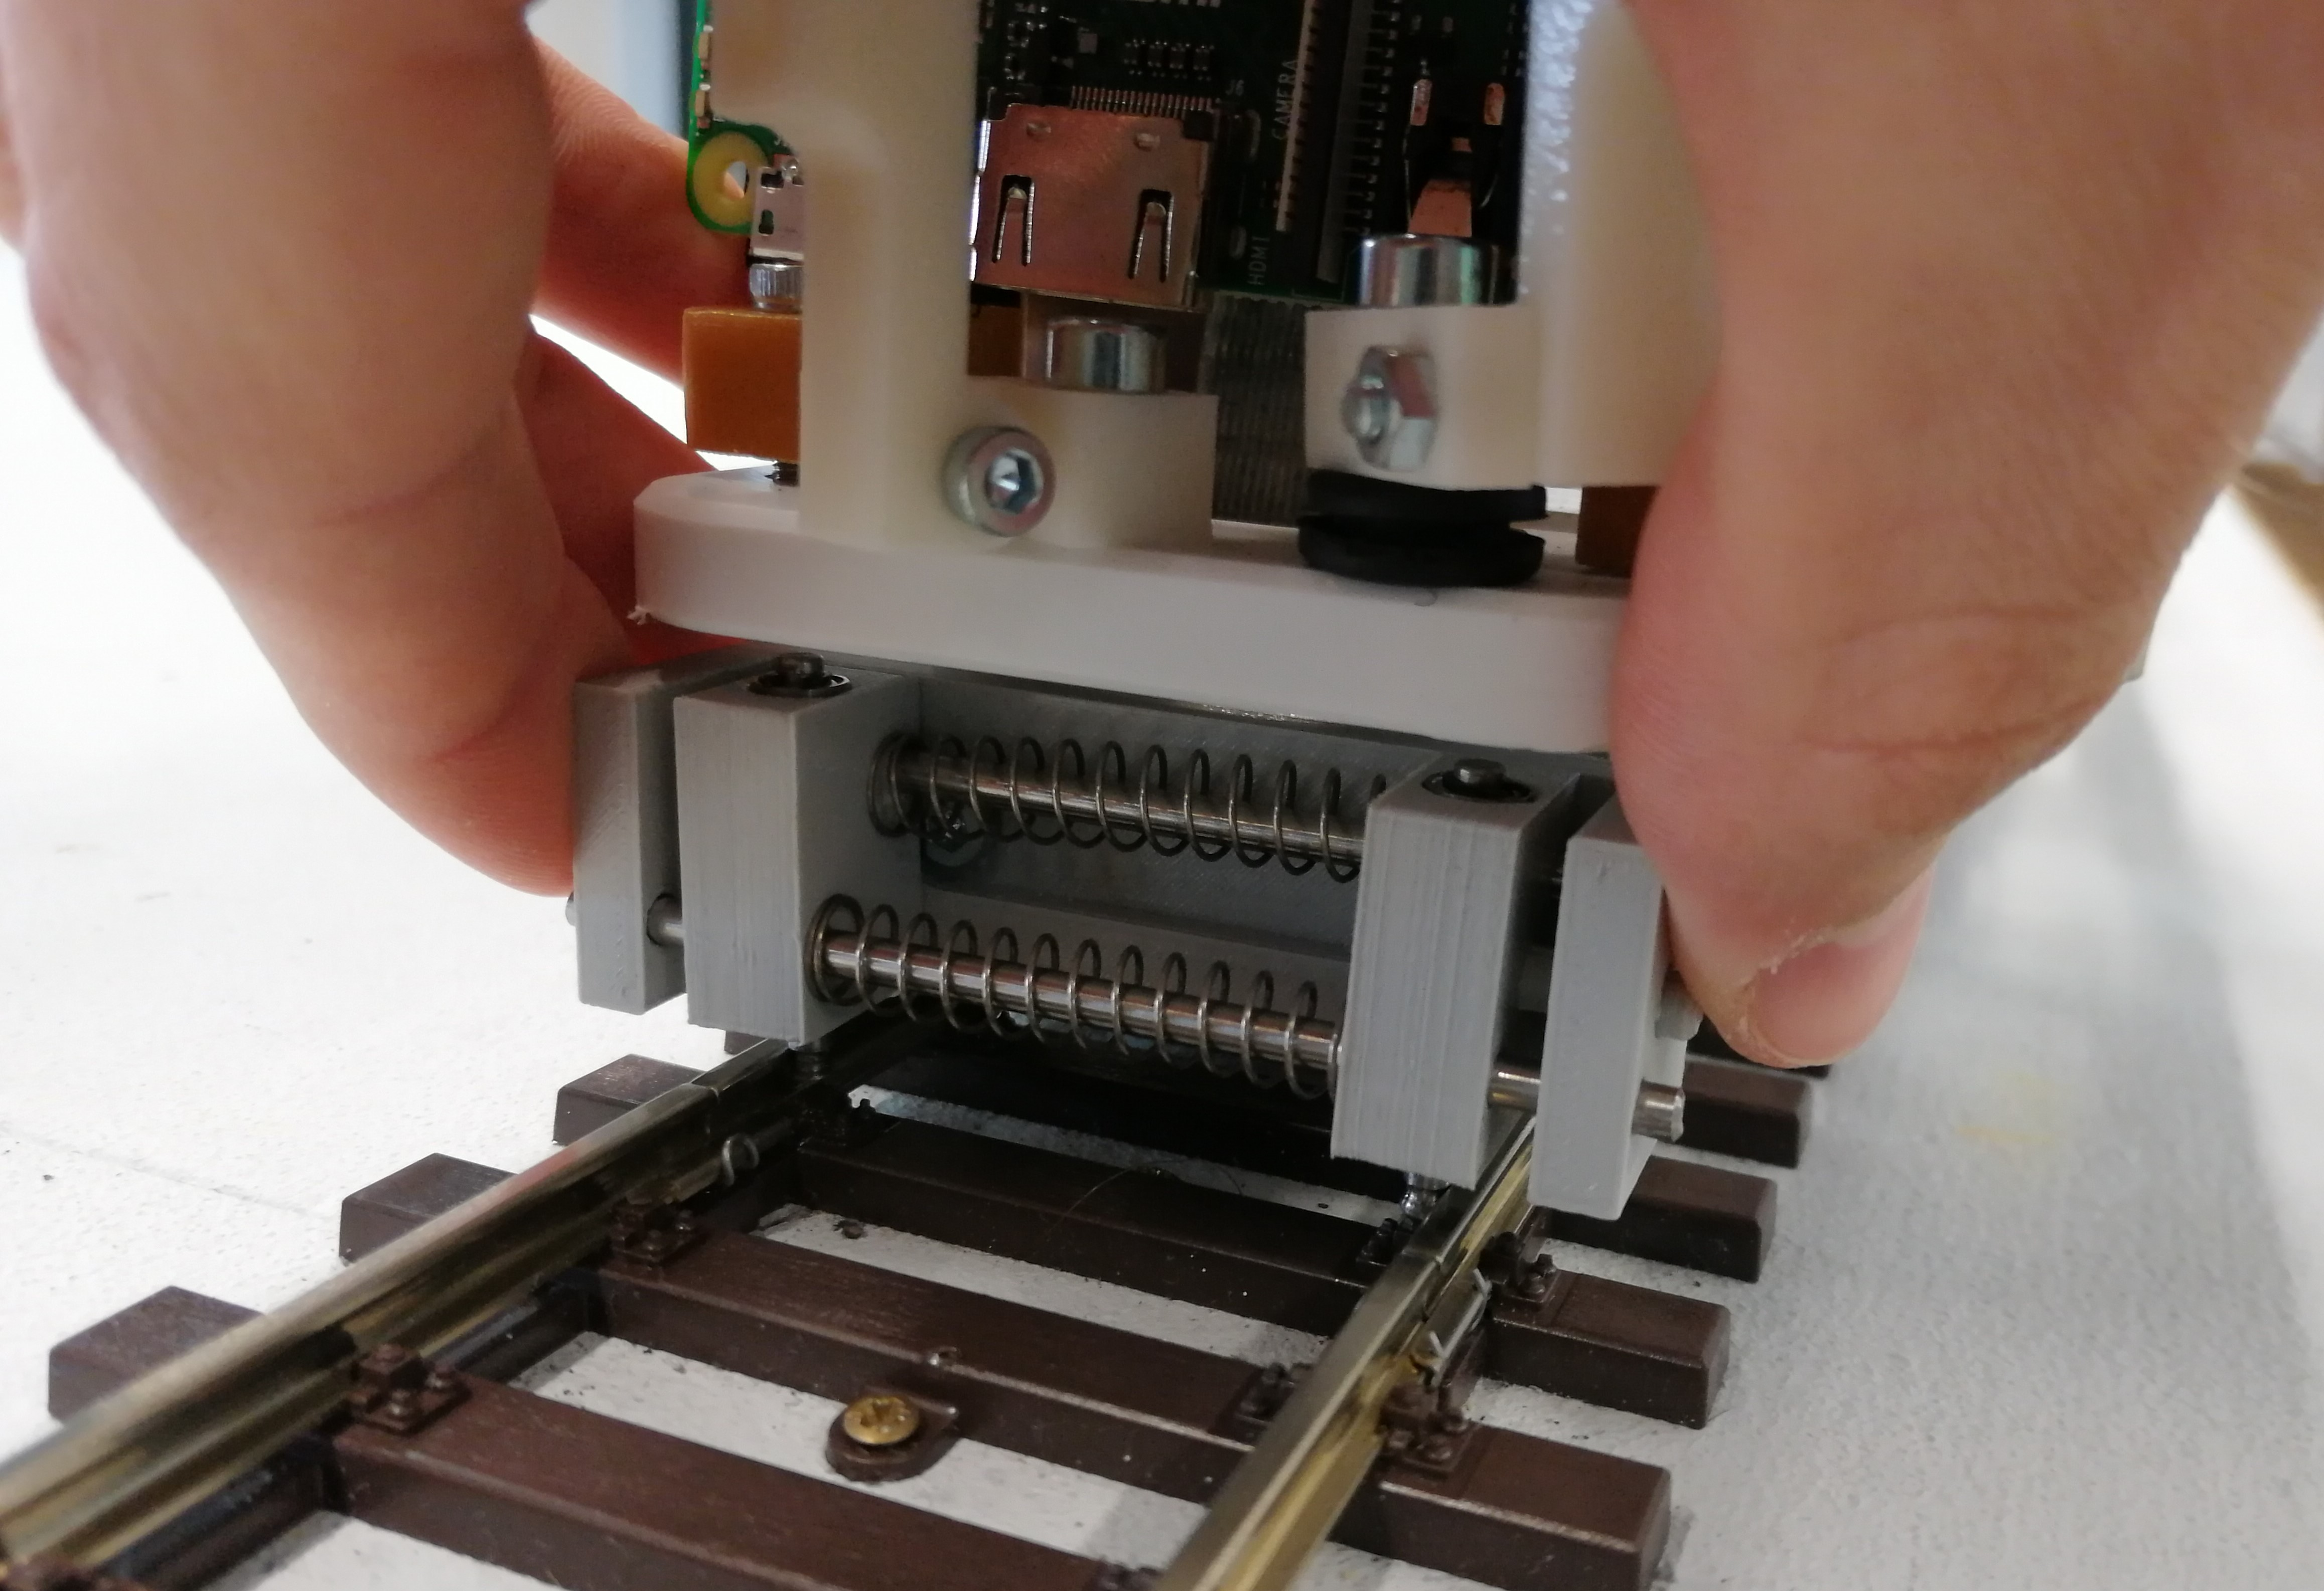
\includegraphics[width=0.495\textwidth]{../../images/Maschinentechnik/montagevorne.PNG}
  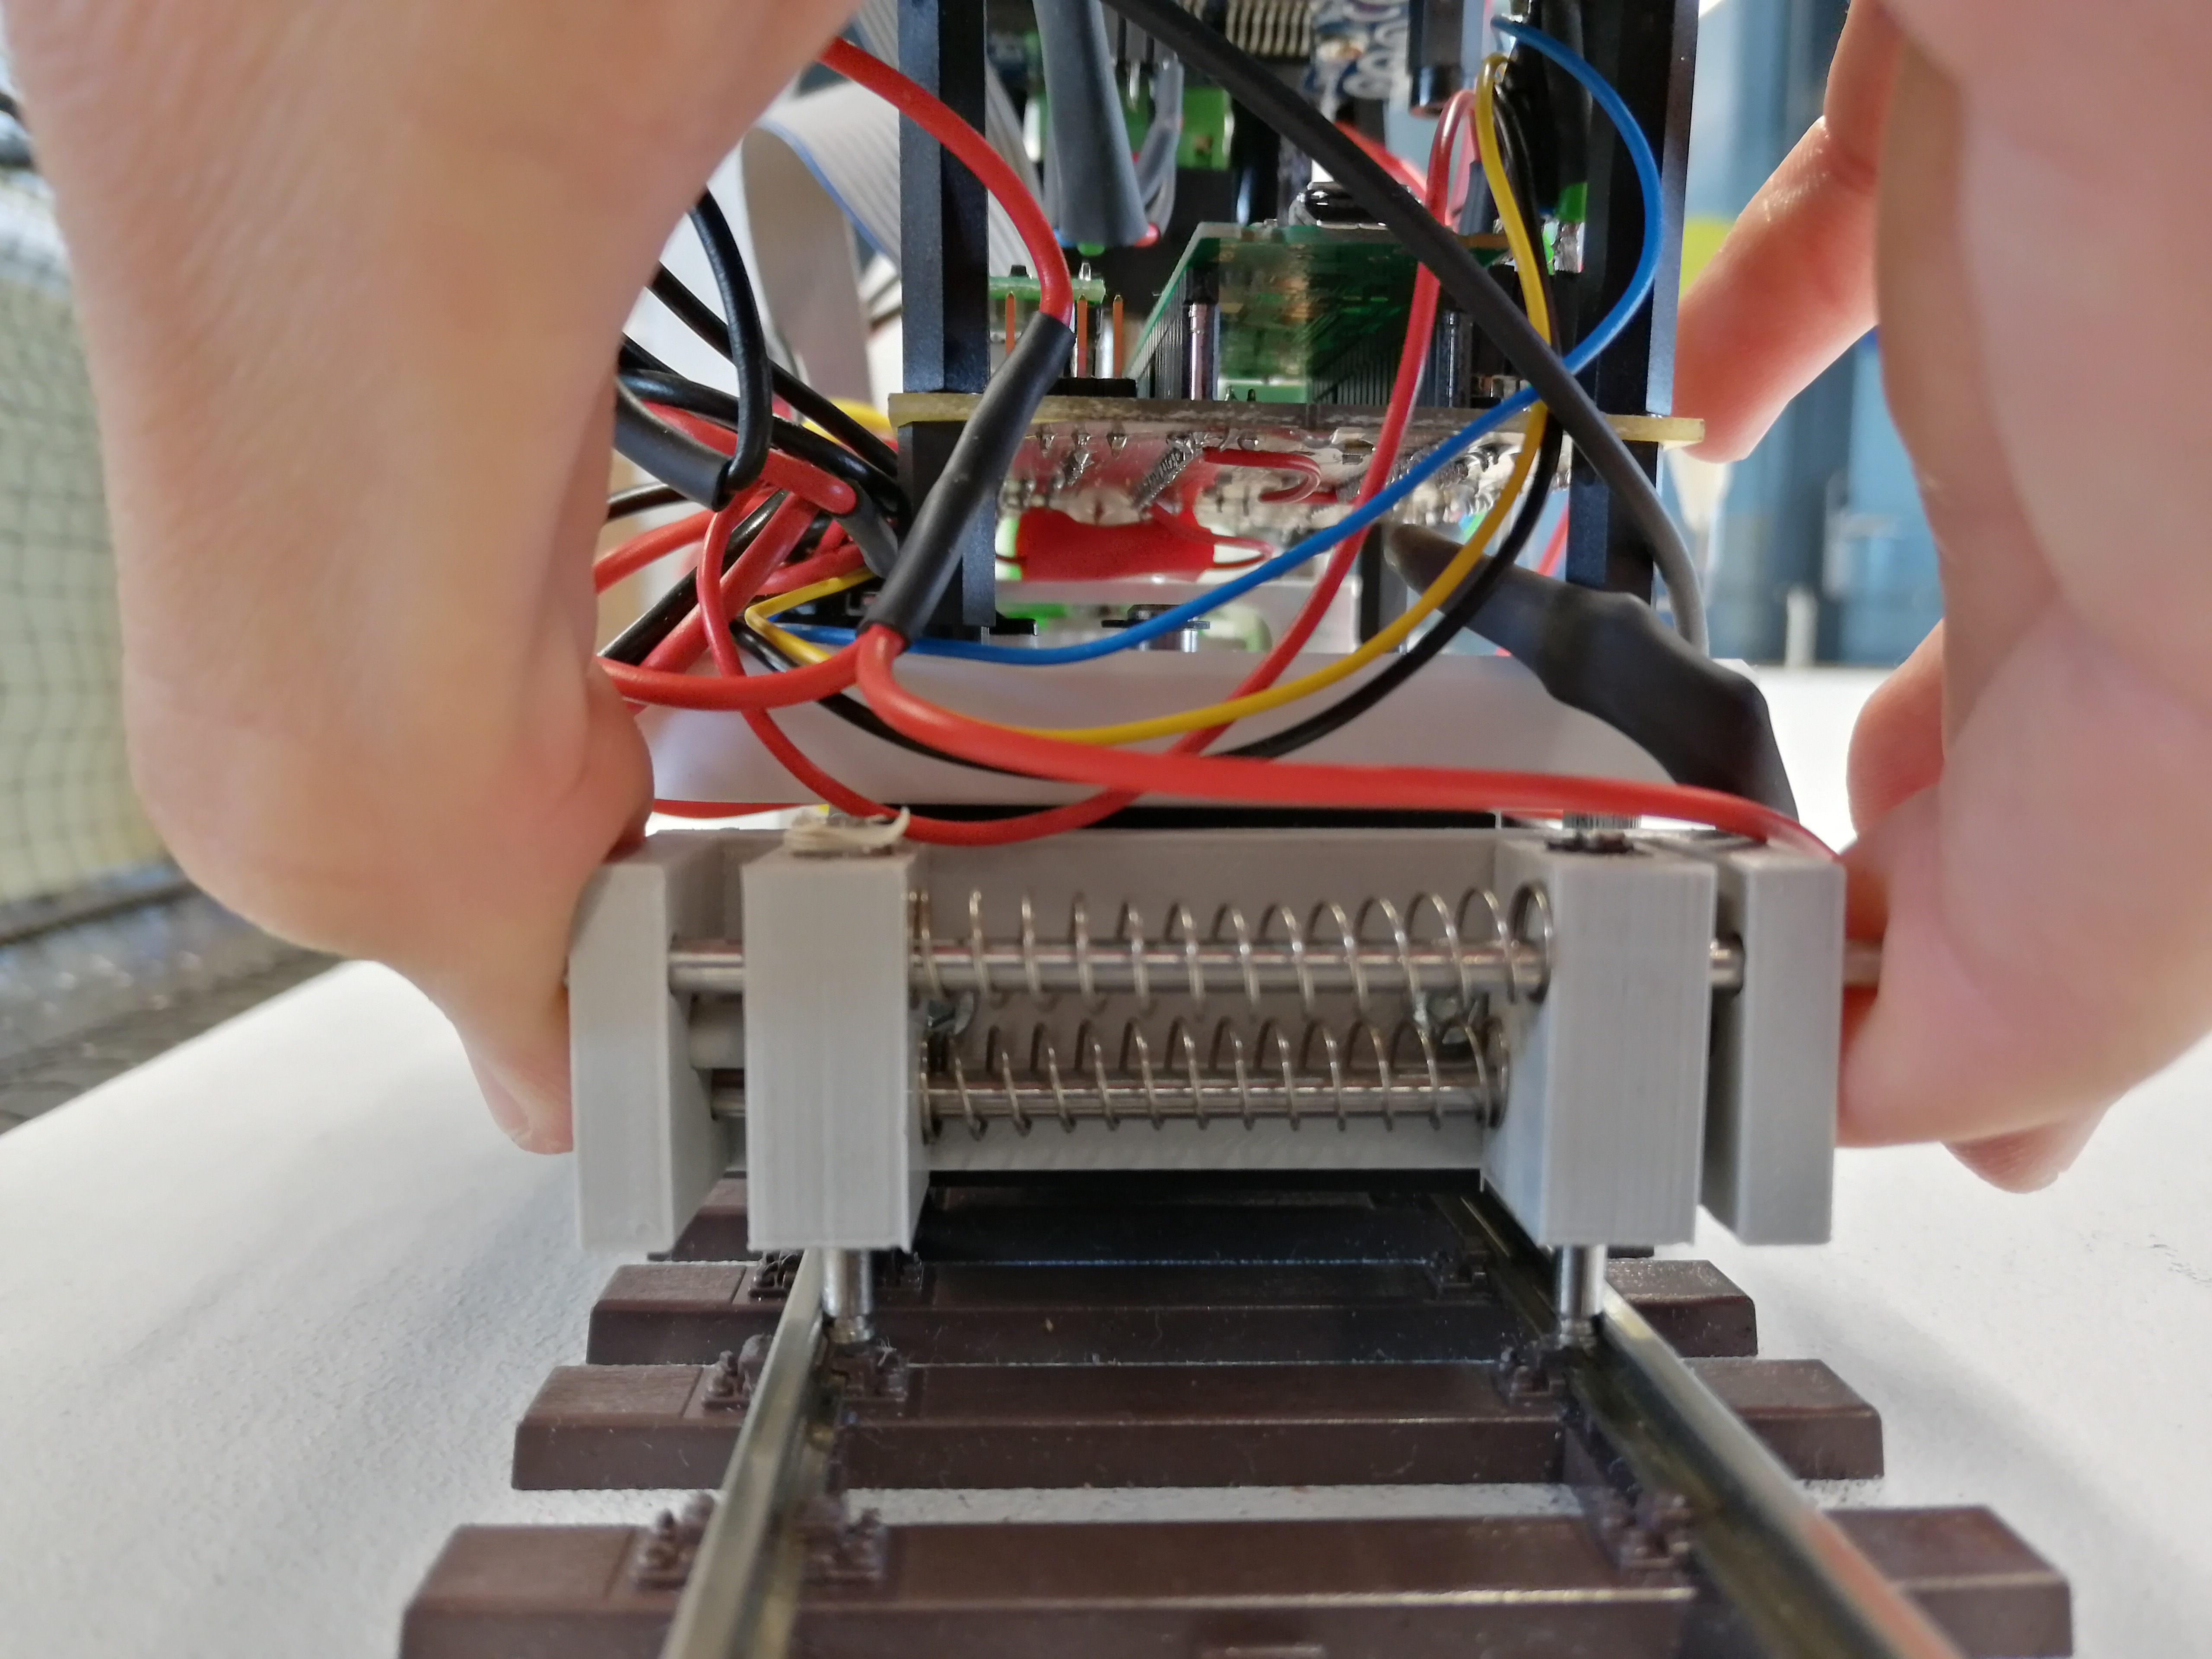
\includegraphics[width=0.455\textwidth]{../../images/Maschinentechnik/montagehinten.PNG}
  \caption {Kurvenvorrichtung vorne und hinten von der Lokomotive einhacken}
\end{figure}

\newpage

\textbf{3. Kranhebel in die Ausgangslage bringen}\\
In diesem Teilschritt soll sichergestellt werden, dass der Kranhebel ausgefahren und an der Startposition platziert ist. Dafür drückt man den Hebel, welcher in Richtung mittelpunkt der Teststrecke zeigt, an den Anschlag unten.\\

\begin{figure}[H]
  \centering
  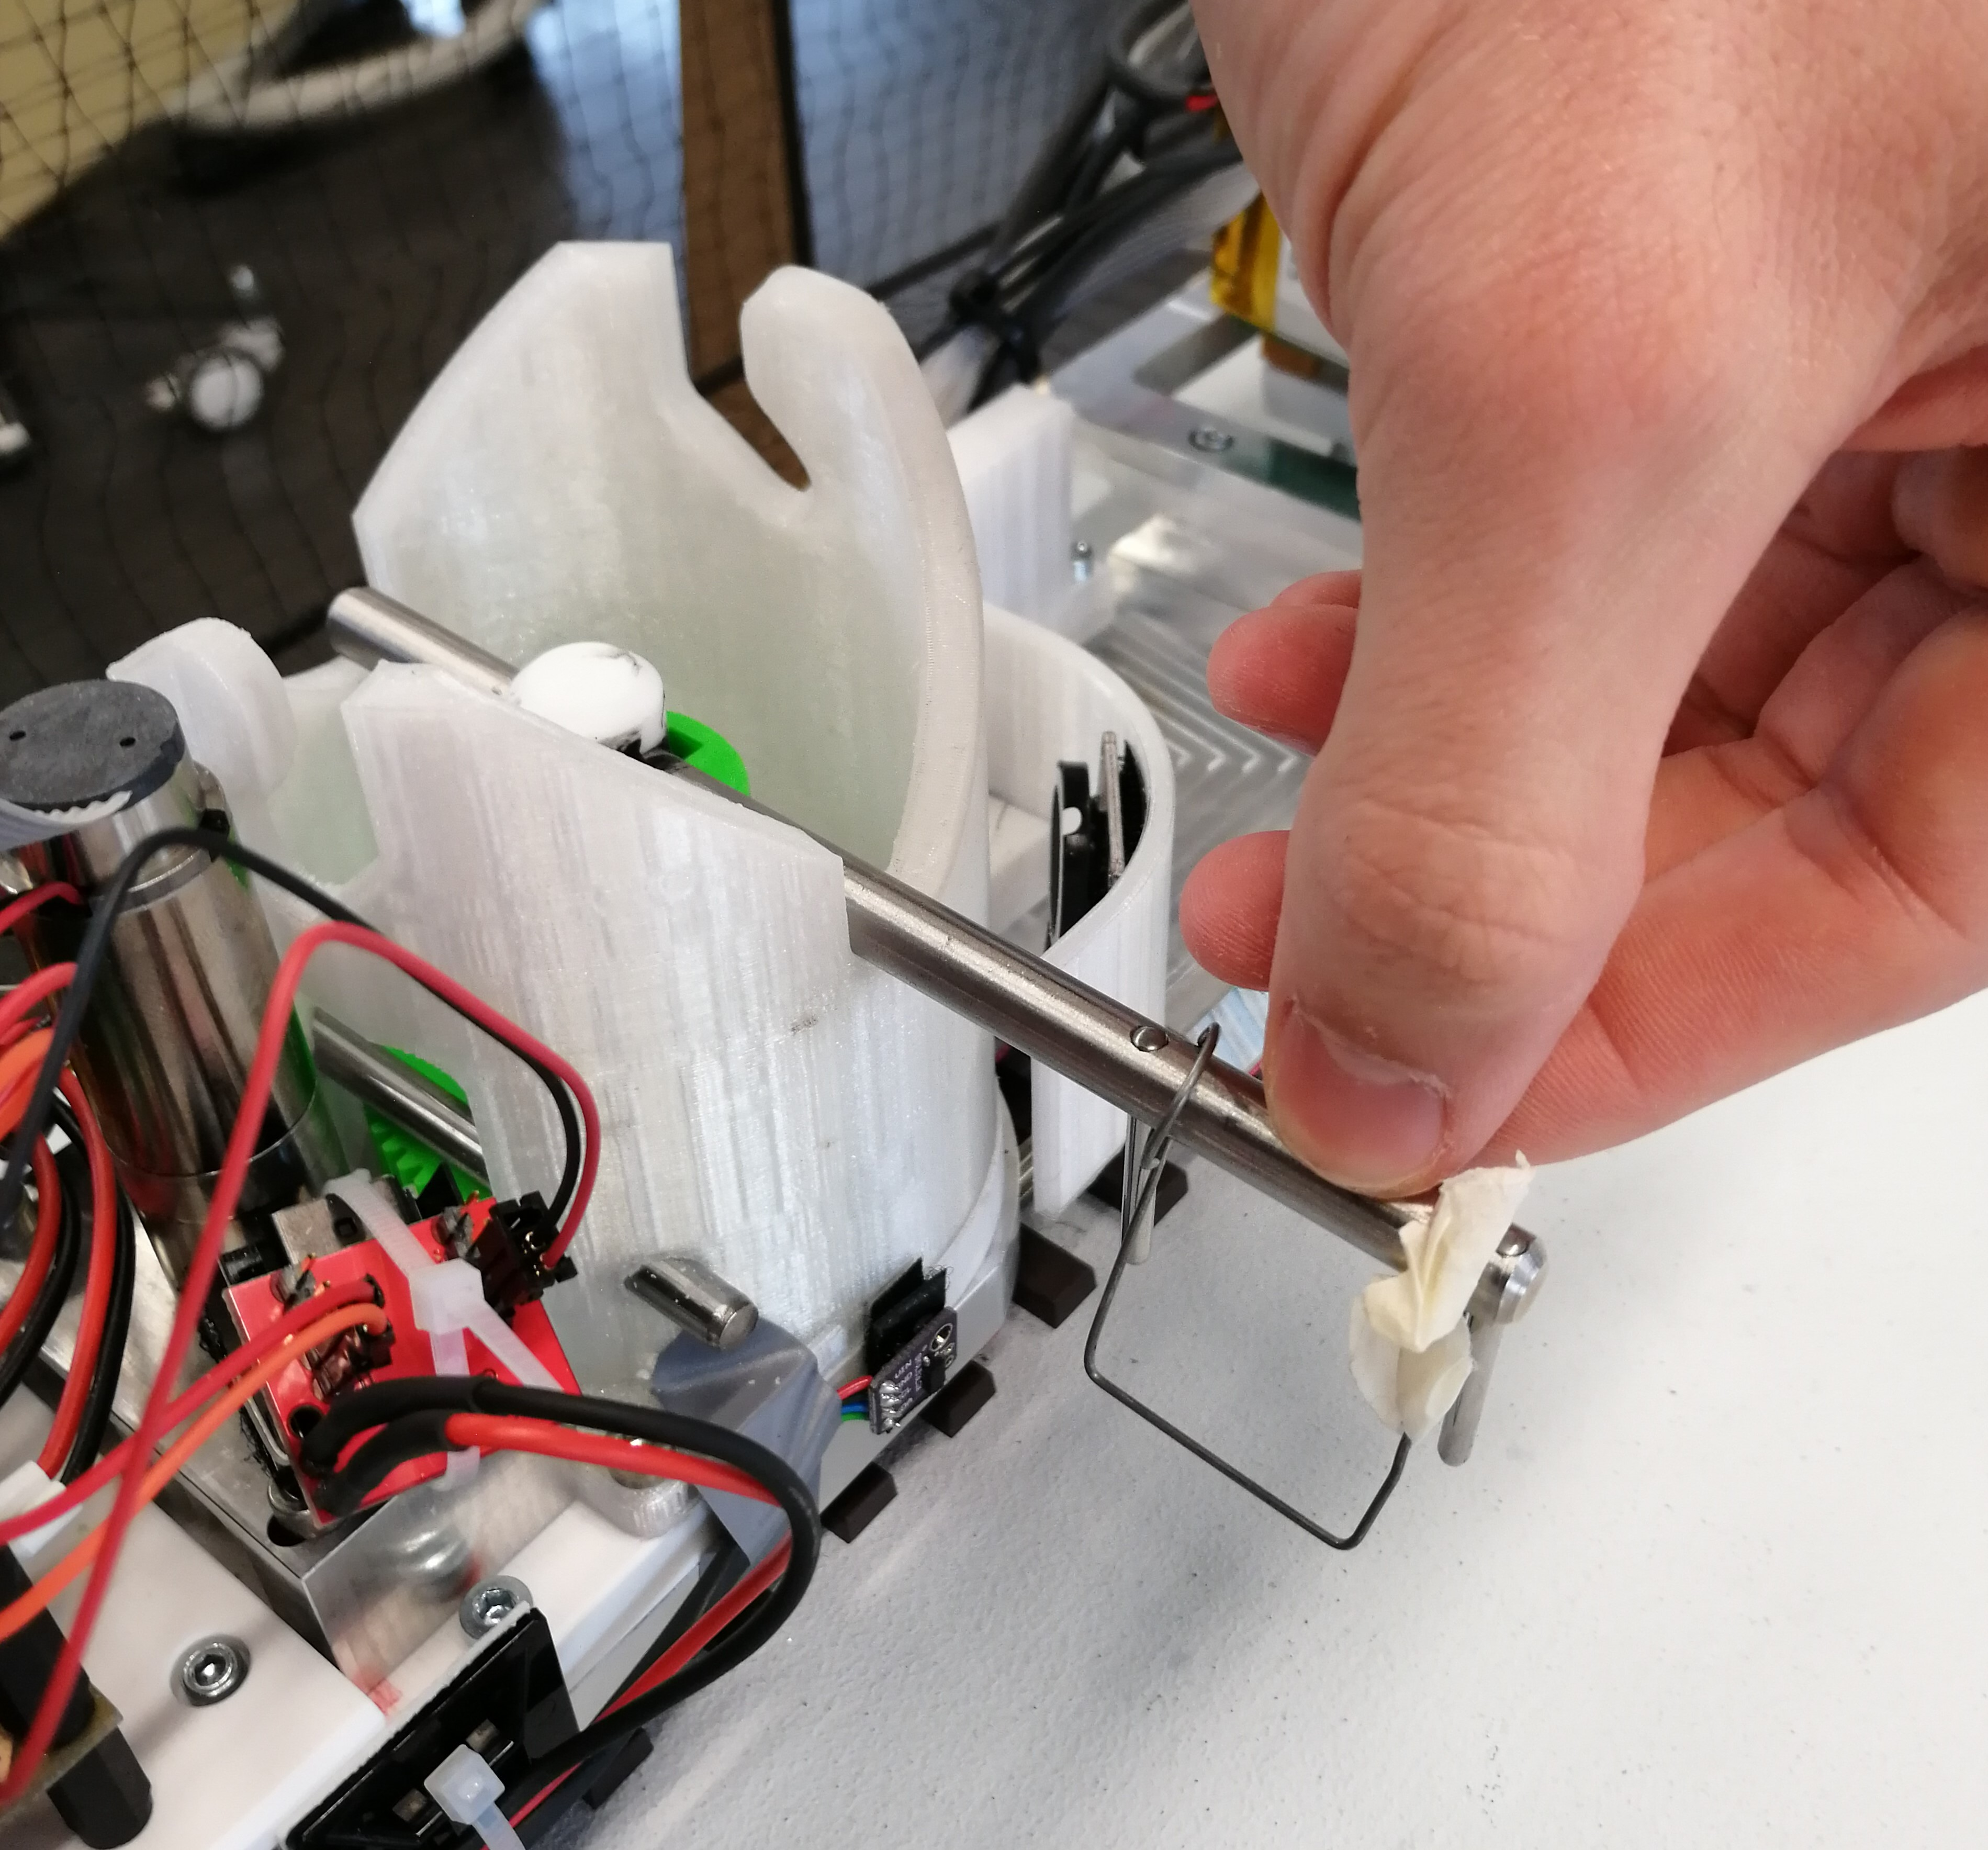
\includegraphics[width=0.5\textwidth]{montagekran.PNG}
  \caption {Lokomotive auf Gleis}
  \label{fig:montagezug}
\end{figure}

\textbf{4. Kontrolle und Freigabe des Startvorgangs}\\
Am Ende soll nochmals kontrolliert werden, ob die Lokomotive korrekt auf den Rädern aufliegt, alle Schleifkontakte die Gleise berühren und die Kurvenvorrichtung korrekt eingehackt ist. Anschliessend kann die Freigabe für den Startvorgang erfolgen.

\end{document}